\section{Overview}
\label{sec:management_overview}

\begin{figure}[H]
  \hspace*{-2.5cm}
    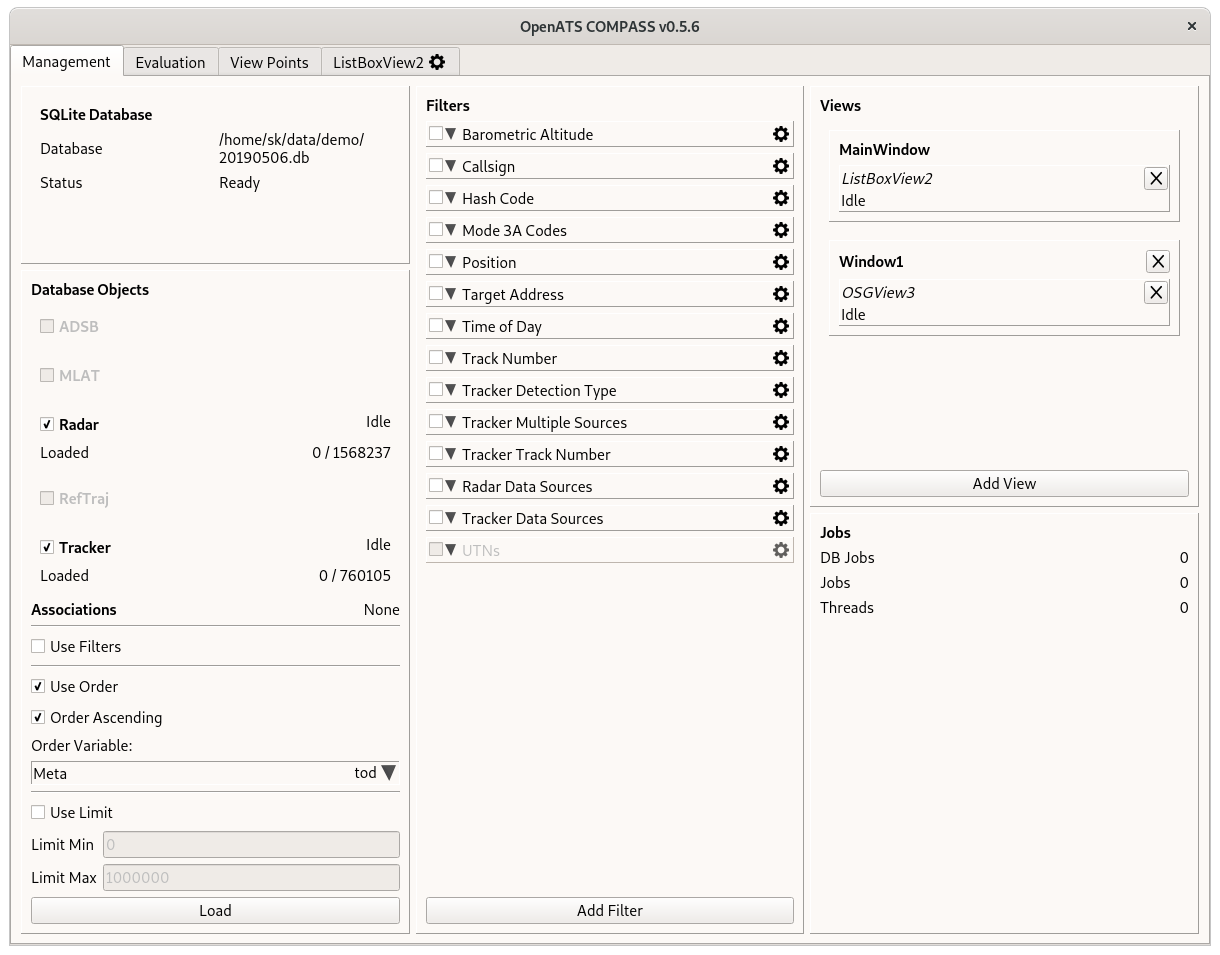
\includegraphics[width=19cm]{../screenshots/management.png}
  \caption{Management window}
\end{figure}

In the uppermost part, the current tab can be selected. In addition to the 'Management' and 'View Points' tabs, views can be added to main window, per default a ListBox view exists. \\

The 'Management' tab shows general database information, a list of database objects with loading functions, a filter system and so on. \\

The 'View Points' tab shows view points and allows for associated functions. For more information please refer to \nameref{sec:view_points}.

\subsection{Database Information}

In this widget, general information about the database is given. 

\begin{figure}[H]
  \center
    \includegraphics[width=8cm,frame]{../screenshots/management_database.png}
  \caption{Management: Database Information}
\end{figure}

This also includes the database status.

\subsection{Database Objects}
\label{sec:management_dbos}

In this widget, information about the DBObjects, the loaded dataset, and the loading parameters are given.

\begin{figure}[H]
  \center
    \includegraphics[width=8cm,frame]{../screenshots/management_dbos.png}
  \caption{Management: DBObjects}
\end{figure}

Each existing DBObject is listed, and active ones have the following items:

\begin{itemize}
 \item Name checkbox: Defines whether data from this DBObject should be loaded
 \item Loading status information
  \begin{itemize}
  \item Idle: Nothing to do at the moment
  \item Loading: DBObject read/write in progress
  \end{itemize}
 \item Loaded data size: Number of loaded items / Number of existing items
\end{itemize}
\ \\

If a DBObject exists, but has no data in the database, it is shown as inactive (greyed out, like ADSB and MLAT in the screenshot).\\

The following important elements exits:
\begin{itemize}
 \item 'Associations' label: Indicates if association information exists, and from which data source
 \item 'Use Filters' checkbox: Whether filtering should be performed
\end{itemize}
\ \\

Additionally, parameters which configure the loading process exist:

\begin{itemize}
\item The following elements should not be used (exist for testing purposes):
\begin{itemize}
 \item 'Use order' checkbox: Whether the dataset should be ordered by a DBO variable
 \item 'Use Ascending' checkbox: If ordered, defines if it should be ascending or descending
 \item 'Order Variable' selection: If ordered, what variable should be used.
\end{itemize}
 \item 'Use Limit' checkbox: If the data size should be limited
 \item 'Limit Min': If limited, the data set will start at the n-th index given here. If 0, it will be loaded from the beginning, if e.g. 100, the first 100 entries will be skipped and the 101st entry will be the first in the dataset.
\item 'Limit Max': If limited, the number given here will be the number of loaded entries.
\end{itemize}
\ \\

Using the 'Load' button, a loading process using the current configuration is started.  \\

When a loading process is in progress, the button displays 'Stop' and can be used to abort the current loading process. Please note that aborting can take a few seconds during which the button is inactive, after successful abort the button states 'Load' and is usable again.

\subsection{Filters}

\begin{figure}[H]
  \center
    \includegraphics[width=7cm,frame]{../screenshots/management_filters.png}
  \caption{Management: Filters}
\end{figure}

Each filter consists of a checkbox, defining if a filter is active (contributes to the search query), a triangle-button (to show/hide the filter configuration elements), a unique name, and a manage button (activates a context menu). At the bottom an 'Add filter' button exists, which can be used to add new filters. \\

Please \textbf{note} that the filter configuration will be saved at program shutdown, which is also true for new filters.   At  startup,  all  filters  from  the  configuration  are  generated  and  restored  to  their  previous  state. However, when the database was changed (usage of different data source), all filters are reset to an initial
state (since their previous configuration may be senseless). \\

Please also \textbf{note} that active filters, at the moment, are always combined with a logical AND. Therefore,
when  two  filters  are  active,  only  the  intersection  of  data  which  both  filters  allow  is  loaded.   A  logical combination of filters using an OR operation is planned, but was not implemented yet.

\subsubsection{Data Source Filters}
For each DBO with a data sources list, a data source filter is generated which can not be edited or deleted.  For each
data source a checkbox exists, which is only active if the data source was active in the database. If checked, the
data generated by the data source is loaded, and otherwise not.

\subsubsection{Custom filters}
A  custom  filter  does  not  differ  in  general  usage,  but  the  inner  workings  are  different.   Also,  it  can  be generated using the 'Add filter' button. It can also be reset (to the original values) edited and deleted using
the manage button. \\
A custom filter consists of one or more filter conditions.  Such a condition involves a DBO (or meta) variable, an operator, and a value.  When active, the filter restricts all loaded DBO data to be fullfill all filter conditions.
As an example, the 'Time of Day' filter limits the loaded data to a specific time window, to load only time slices of the dataset.  The 'Mode 3A Codes' filter restricts to a list of (comma-separated) Mode 3/A codes, to single out specific flights. \\

For more information about filtering, please refer to Section \nameref{sec:filtering}.

\subsection{Views}

\begin{figure}[H]
  \center
    \includegraphics[width=8cm,frame]{../screenshots/management_views.png}
  \caption{Management: Views}
\end{figure}

This element allows generation and management of all active Views and windows. Each View is contained
in a tab within a parent window.  At startup, only the main window exists ('MainWindow'), which also holds
the management tab. If the main window is closed, the COMPASS client shuts down. New Views can be added using the 'Add View' button, which opens a pull-down menu. Each View can either be added to the main window ('MainWindow') or into a new window. When added, a new tab exists in the containing window, and controlling elements are added for any new
windows or views. \\

New Views can be added either to currently existing windows as new tabs, or to a newly opened window. A window can be closed either by the close button in the window decoration, which discards all contained Views within the window.  To delete a single View, one can use the close button in the GUI, which frees up all its allocated resources. Each View adds its required variables to the loading list for the database.  During a loading process, the loading status  of a View is shown in the management tab.\\

Currently, the following Views exist:
\begin{itemize}
 \item \nameref{sec:listbox_view}
 \item \nameref{sec:osg_view}
\end{itemize}


\subsection{Jobs}

The COMPASS framework supports multi-threading. A number of processing steps ('Jobs') can be exectuted on a number of parallel threads. Since multi-threading on a database creates limited benefit, only one thread is used specifically for database jobs. All non-database jobs are exectuted on a dynamic number of other threads, which are increased/decreased in number depending on the application's needs. 

\begin{figure}[H]
  \center
    \includegraphics[width=8cm,frame]{../screenshots/management_jobs.png}
  \caption{Management: Jobs}
\end{figure}

In the Job element the number of database jobs is listed under 'DB Jobs', the number of other Jobs is listed under 'Jobs'. The number of active processing threads is listed under 'Threads'.
 
